\documentclass[11pt]{article}

\usepackage{float}
\usepackage[T1]{fontenc}
\usepackage{lmodern}
\usepackage{caption}
\usepackage{subcaption}
\usepackage[colorlinks=true]{hyperref}
\usepackage[backend=biber]{biblatex}

\addbibresource{references.bib}

% Margins
\usepackage{geometry}
\geometry{
   % includeheadfoot,
   margin=2.54cm
}

% Code highlighting
\usepackage{minted}
\newminted[code]{Haskell}{
  xleftmargin=1em
}
\newminted[agcode]{Haskell}{
  xleftmargin=1em
}

% Graphics
\usepackage{graphicx}
\graphicspath{ {./images/} }

\usepackage{parskip}

\author{
  Jaro Reinders\\ Eindhoven University of Technology \\
  \\
  Supervised by:
  \vspace{0.5em}\\
  \begin{minipage}[t]{.4\textwidth}
    \centering
  Jurriaan Hage\\
  Utrecht University
  \end{minipage}%
  \begin{minipage}[t]{.4\textwidth}
    \centering
  Tom Verhoeff\\
  Eindhoven University of Technology
  \end{minipage}
}

\title{Mirage: Attribute Grammar Visualization}

\begin{document}

\maketitle

\begin{abstract}
  In this report I describe the results of my internships at Utrecht University in which I developed a visualization tool for attribute grammars. Attribute grammars are used to define tree traversals which are often used in compilers. Their modular nature grants their users much freedom, but it can also make it harder to see how all the components interact. To address this I have developed a visualization tool called Mirage in the Haskell programming language. I describe the design and implementation and discuss how it improves on a previous visualization tool called Visage which has not seen much use in practice. For the implementation of Mirage I have used attribute grammars and experimented with writing graphical interfaces in Haskell. With Mirage I hope to contribute a tool that can really be used in practice to understand attribute grammars and make developing them easier. Finally, in this report I suggest many extensions and improvements that could be implemented in future projects. The source code can be found at \url{https://github.com/Helium4Haskell/mirage}.
\end{abstract}

\newpage

\tableofcontents

\newpage

\section{Introduction}

This report is part of my internship at the University of Utrecht in the first term of academic year 2020-2021. I am interested in the attribute grammar system developed at Utrecht University and thought the documentation and usability of the system could be improved. Jurriaan suggested that I could work on a visualizer for these attribute grammars and this would also allow me to learn a bit more about the internal workings of the system. Additionally, this internship has given me a taste of what working at the software technology research group at the University of Utrecht is like. I am grateful for the warm welcome I have received despite the current COVID-19 pandemic. The requirements for this project were mostly defined by Jurriaan Hage who wants to use this visualizer for visualizing attribute grammars of the Helium compiler that he works on.

In the introduction of this report I assume that the reader has some basic knowledge of programming in Haskell to motivate attribute grammars. I explain the syntax and semantics of the Utrecht Univsersity Attribute Grammar system where I use it, but for a more complete description I would recommend the reader to consult the latest manual\footnote{\url{http://www.cs.uu.nl/docs/vakken/mapa/downloads/agmanual.pdf}}.

Let us begin by looking at a common use case to motivate attribute grammars.
Compilers often perform many traversals of abstract syntax trees.
For that purpose compiler writers can use general purpose programming languages, such as the functional programming language Haskell.
Consider the following small arithmetic expression language with constants, addition and variables.

\begin{code}
data Exp = Con Int | Add Exp Exp | Var Name
\end{code}

Here we assume that \mintinline{Haskell}{Env} is some data type that contains variable bindings which can be queried with \mintinline{Haskell}{lookup :: Env -> Name -> Int} and \mintinline{Haskell}{Name} is a string that contains the name of a variable.

A possible semantics of this language can be expressed as a function that takes in an environment that holds the value of each variable and produces the result of performing the arithmetic operations. In Haskell those semantics can be written as follows.

\begin{code}
semExp1 :: Exp -> Env -> Int
semExp1 (Con con)     _   = con
semExp1 (Add lef rit) env = semExp1 lef env + semExp1 rit env
semExp1 (Var name)    env = lookup env name
\end{code}

For small languages this approach is perfectly adequate. But this approach starts to become much more complicated for larger languages. For example, we can extend the arithmetic expression language by adding a second return type which aggregates all the variables that have been encountered during the traversal.

\begin{code}
semExp2 :: Exp -> Env -> (Int, [Name])
semExp2 (Con con)     _   = (con, [])
semExp2 (Add lef rit) env = let ~(lefVal, lefVars) = semExp2 lef env
                                ~(ritVal, ritVars) = semExp2 rit env
                            in (lefVal + ritVal, lefVars ++ ritVars)
semExp2 (Var name)    env = (lookup env name, [name])
\end{code}

Notice that this one small change which is conceptually independent from most of the existing code has forced us to rewrite the entire function. Additionally, in the right hand side of the \mintinline{Haskell}{Add} case you can see that we need to write boilerplate code for unpacking the results of the children and wrapping the result in a tuple again after computing the results.

In real-world compilers, such as the Helium Haskell compiler~\cite{helium} there can be many nested data types with dozens of constructors and the semantics can involve dozens of input and dozens of output variables. For such use cases it is clear that there is a need for another approach.

Attribute grammars~\cite{knuth-attribute-grammars} as implemented in the University of Utrecht Attribute Grammar Compiler (UUAGC)~\cite{uuagc} offer a compelling solution to this problem in the form of a domain specific language for describing these tree traversals. The main insight is to define the input and output variables separately for a data type and also allow implementing their semantics separately. The equivalent of the above \mintinline{Haskell}{Exp} type and the \mintinline{Haskell}{semExp1} semantics are given by attribute grammar shown in Figure~\ref{arith-ag}.

\begin{figure}[h]
\begin{agcode}
data Exp
  | Con  con  :: Int
  | Add  lef  :: Exp   rit :: Exp
  | Var  name :: Name

attr Exp
  inh env :: Env
  syn val :: Int

sem Exp 
  | Con lhs.val = @con
  | Add lhs.val = @lef.val + @rit.val
        lef.env = @lhs.env
        rit.env = @lhs.env
  | Var lhs.val = lookup @name @lhs.env
\end{agcode}
  \caption{Attribute grammar of a simple arithmetic expression evaluator.}
  \label{arith-ag}
\end{figure}

At the top we see the data definition which is very similar to standard Haskell notation except that we give a name to each of the children. Below that there is an attribute definition which is entirely new. Two attributes are declared, one inherited (input) attribute and one synthesized (output) attribute. Finally, at the bottom you can see the semantic rules. Instead of defining one equation per constructor we define equations for each attribute of each constructor. Introducing a new attribute can now be done without changing any of the existing code. The code that needs to be added is shown in Figure~\ref{arith-vars-ag}.

\begin{figure}[h]
\begin{agcode}
attr Exp
  syn vars :: {[Name]}

sem Exp
  | Con lhs.vars = []
  | Add lhs.vars = @lef.vars ++ @rit.vars
  | Var lhs.vars = [@name]
\end{agcode}
  \caption{Extending the simple arithmetic evaluator to also collect all used variables.}
  \label{arith-vars-ag}
\end{figure}

UUAGC will take all these definitions and combine them into a Haskell function that is very similar to \mintinline{Haskell}{semExp2}. This makes it easier for developers to extend their tree traversals. But, it also comes with downsides. Splitting up code can make it harder for people who read the code to get a complete picture of which attributes belong to which nonterminals.

To address this issue, Tim Adelaar and Jurriaan Hage developed an attribute grammar visualization tool called Visage.
The idea of Visage is to hook into UUAGC, capture the grammar that UUAGC gathers from the source code files and visualize it for the programmer.

\begin{figure}[H]
  \center
  \begin{subfigure}[b]{0.45\textwidth}
    \centering
    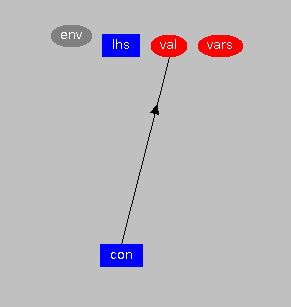
\includegraphics[scale=0.7]{exp-con-visage}
    \caption{The \mintinline{Haskell}{Con} production.}
    \label{exp-con-visage}
  \end{subfigure}
  \hfill
  \begin{subfigure}[b]{0.45\textwidth}
    \centering
    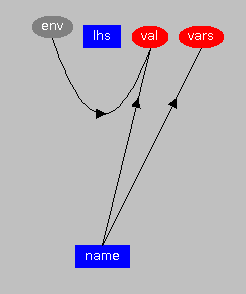
\includegraphics[scale=0.7]{exp-var-visage}
    \caption{The \mintinline{Haskell}{Var} production.}
    \label{exp-var-visage}
  \end{subfigure}

  \vspace{1em}
  \begin{subfigure}[b]{\textwidth}
    \centering
    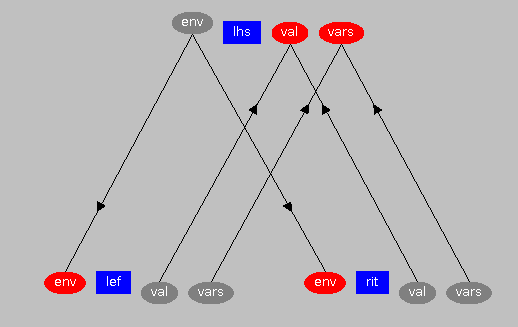
\includegraphics[scale=0.7]{exp-add-visage}
    \caption{The \mintinline{Haskell}{Add} production.}
    \label{exp-add-visage}
  \end{subfigure}
  \caption{Visualization of the extended arithmetic expression language created by Visage.}
\end{figure}

For this visualization, Visage uses the layout that is commonly drawn on a blackboard or shown on the slides of lectures on the subject of attribute grammars. Every production rule, from now on abbreviated to production, is visualized separately. At the top of each visualization is always a node called ``lhs'' (left hand side) with on its left the list of inherited attributes which are the inputs of this production and on the right the list of synthesized attributes which are the output of this production. At the bottom the children are visualized. There are terminal children which do not have any attributes and represent plain Haskell values. For example \mintinline{Haskell}{con} in Figure~\ref{exp-con-visage} and \mintinline{Haskell}{name} in Figure~\ref{exp-var-visage}. And there are nonterminal children with their own inherited attributes on the left and synthesized attributes on the right. Examples of nonterminal children are \mintinline{Haskell}{lef} and \mintinline{Haskell}{rit} in Figure~\ref{exp-add-visage}. Note that the input and output attributes are swapped for the children: we need to define their inherited attributes and we can use their synthesized attributes. Arrows between the attributes indicate a dependency relation.

Unfortunately, Visage has not seen widespread use due to some major drawbacks.
First and foremost is the problem of scaling.
The visualization itself can become too big to fit on the screen at once.
This can be seen in a real world example in Figure~\ref{big-visage}.
We can see that Visage can only visualize at most about 20 attributes of the lhs or of all the children combined.
And the time required to load a new grammar can get quite long for large grammars. Visage uses a mostly custom data interchange format based on ATerms~\cite{aterms}. Additionally, Visage extracts dependency information from the rule implementation code snippets when loading a grammar file. These are all factors that might cause this slowdown.

\begin{figure}[h]
  \centering
  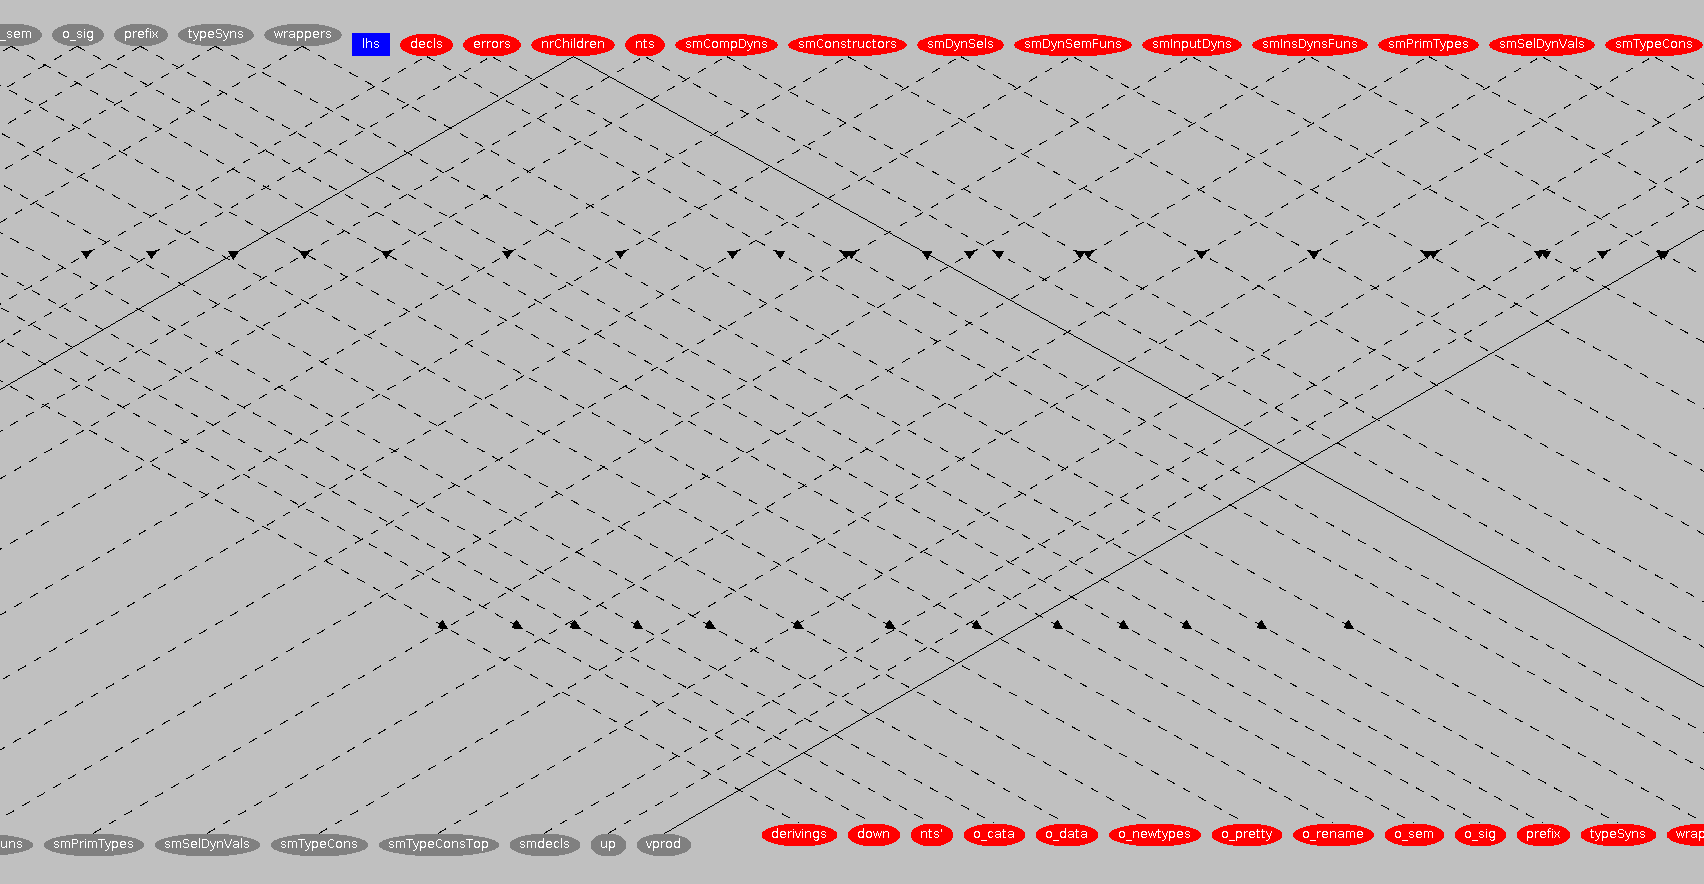
\includegraphics[width=\linewidth]{big-visage}
  \caption{An example with too many attributes to fit on the screen when visualized with Visage.}
  \label{big-visage}
\end{figure}

Another big disadvantage is the lack of maintainability. Visage consists of about 3000 lines of Java source code distributed over 50 classes. Previous modifications have required an unreasonable amount of message passing through the class hierarchy to get data from one class to another.
The impedance mismatch between the object-oriented Java code of Visage and the Haskell code with algebraic data types of UUAGC has also hindered maintenance.

In this report we describe Mirage, a new attribute grammar visualization tool.
We have developed it from scratch as a modern replacement of Visage.
Mirage can visualize more complex models on one screen and also do it faster.
Mirage is written in Haskell using popular and well-supported libraries to improve maintainability.

\section{Design}
\label{design}

In this section, we will describe the final design and the choices that were made.
First we discuss features that were already present in the predecessor Visage. Afterwards, we discuss new improvements in Mirage.

\subsection{Implicit dependencies}

An important feature of UUAGC is that it can automatically generate some semantic rules that only copy or combine values. If the user does not provide an explicit rule for an attribute then UUAGC will fall back on a default semantic rule for that attribute. Users can use this feature and leave out semantic rules if they know that it will be generated automatically. But semantic rules can be written in many places, even in different files, so it is important for users to know if their rules are really automatically generated or if they have accidentally overwritten them somewhere else. So, these implicit dependencies are visualized differently from normal dependencies. In Visage this was done with a dashed line. In Mirage we have decided to make implicit dependencies gray instead of the normal black lines.

\begin{figure}[h]
  \centering
  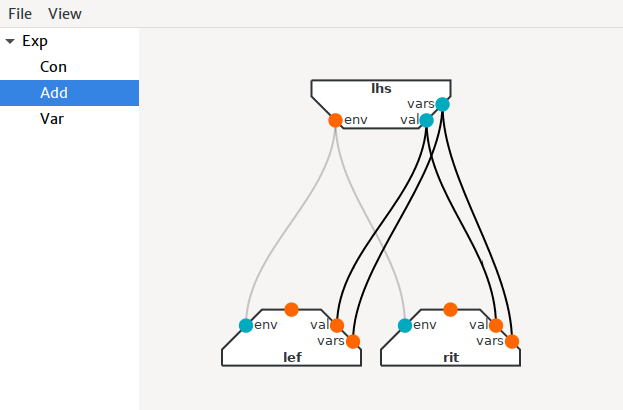
\includegraphics[scale=0.5]{implicit-mirage}
  \caption{Mirage visualization of implicit arguments.}
  \label{implicit-mirage}
\end{figure}

In Figure~\ref{implicit-mirage} we visualize the \mintinline{Haskell}{Add} production of the arithmetic expression language.  We have changed the semantic rules slightly by leaving out the rules for the inherited attribute \mintinline{Haskell}{env}. Leaving out this rule causes UUAGC to automatically generate a copy rule that simply copies the value of \mintinline{Haskell}{env} to the children. The resulting visualization shows the distinction between implicit and explicit rules.

\subsection{Type, code and location information}

To make the visualizations useful for code exploration it is important that the user can get more information about the rule that defines the value of an attribute. In Visage, hovering over an attribute will show its type and clicking on an attribute will open a window at the bottom of the screen that shows the source code and in which file that code is located.

\begin{figure}[h]
  \centering
  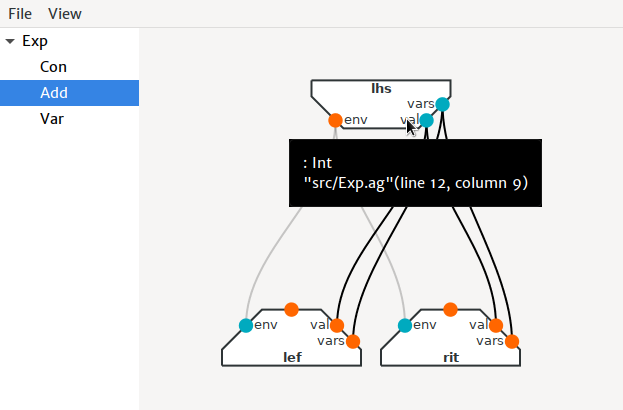
\includegraphics[scale=0.5]{hover-mirage}
  \caption{Mirage visualization of the hover tooltip.}
  \label{hover-mirage}
\end{figure}


In Mirage we have chosen to include the location in the hover tooltip as shown in Figure~\ref{hover-mirage}. The actual source code is shown in a separate window if the user clicks on an attribute. Mirage does not include the source code in the main window at the bottom like Visage, because Mirage uses more of the vertical space for the main visualization as will be explained in Section~\ref{trapezoid}. Users can manually place the source window below the main window if they desire to do so.

\subsection{Filtering attributes}

Showing all information of complex productions onto one screen in a comprehensible way is not possible in general.
Moreover, attribute grammars used in real world applications already run into this problem.
Our main approach to address this problem is to selectively hide information from the user.
The information that grows the most during the development of an attribute grammar are the number attributes, so it makes sense to make it possible to hide attributes.
In Visage a user can hide an attribute by double-clicking on that attribute.
This will cause the attribute name to be hidden, but it still leaves a small ellipse that can be double-clicked to show the attribute again.
An example of this with the running example of the arithmetic expression grammar is shown in Figure~\ref{hidden-visage}.

\begin{figure}[h]
  \centering
  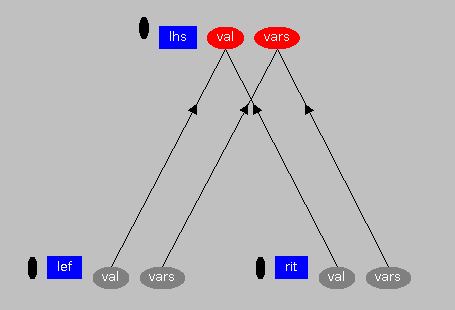
\includegraphics[scale=0.6]{hidden-visage}
  \caption{The \mintinline{Haskell}{Add} rule of the arithmetic expression langauge where the environment is hidden in Visage.}
  \label{hidden-visage}
\end{figure}

There are several disadvantages to this approach. It requires leaving some ellipses on the screen which can take up space, the user does not see the name of the attribute if they want to show it again, and a user that wants to hide a specific attribute must spend some time on trying to locate that attribute especially in larger productions where many attributes fall outside the visible part of the screen.

In Mirage we address these issues by collecting all attributes and displaying them in a list where the user can enable or disable them. This list is shown in a separate window with two columns, one for the disabled attributes on the left and another for the enabled attributes on the right. This filter window is shown in Figure~\ref{filter-window-mirage}. A user can toggle an attribute by clicking on it and that will enable or disable the attribute for all productions. The lists are sorted alphabetically so users can find attributes quickly and the window can be closed after the user has made a selection which does not leave any artifacts that take up space in the main viewing window.

We have extended the filtering functionality to include a mode in which if the user clicks an attribute name then that attribute and all its dependencies will be toggled. This mode can be enabled and disabled by a switch at the bottom of the filter window as shown in Figure~\ref{filter-window-mirage}. It can be used to discover the transitive dependencies by disabling all attributes and then enabling only one attribute and its transitive dependency. It can also be used to hide bigger groups of attributes at a time when too much information is on the screen. 

\begin{figure}[h]
  \centering
  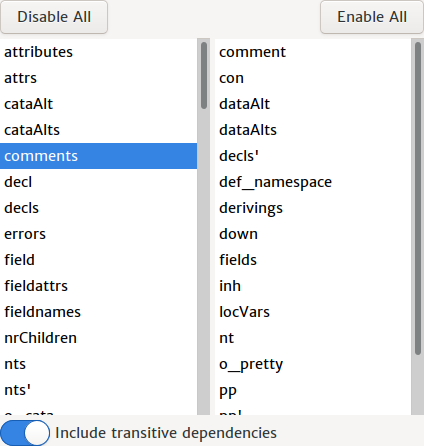
\includegraphics[scale=0.5]{filter-window-mirage}
  \caption{The filter window of Mirage.}
  \label{filter-window-mirage}
\end{figure}

One additional feature in Mirage that also filters attributes is the ``Hide implicit'' toggle. This hides all the attributes that are not used in a currently visible explicit rule. This does not act like a filter. The attributes that are hidden can change if the user selects another production. So, it is more like a post processing filter of the attributes that are shown. Hiding implicit rules like this will reduce the size of the nodes in many cases and in that way it gives more room for other aspects of the visualization such as the explicit dependencies and the local attributes.

\subsection{Diagonal attributes in trapezoidal nodes}\label{trapezoid}

One of the first observations I made was that placing the attribute names next to each other would take up much space. Placing text vertically above each other produces much more compact results, especially for longer attribute names. I initially considered rotating the entire visualization by a quarter turn. But, Jurriaan and I were concerned that rotating everything would be too much of a difference to users that have always used the top to bottom visualization. Jurriaan suggested having all the attributes diagonally aligned such that the attributes are still closely packed together and it is still possible to draw lines straight up or down from the attribute. In Figure~\ref{big-mirage} we can see that Mirage is able to neatly visualize productions that do not fit on one screen when visualized with Visage.

\begin{figure}[h]
  \centering
  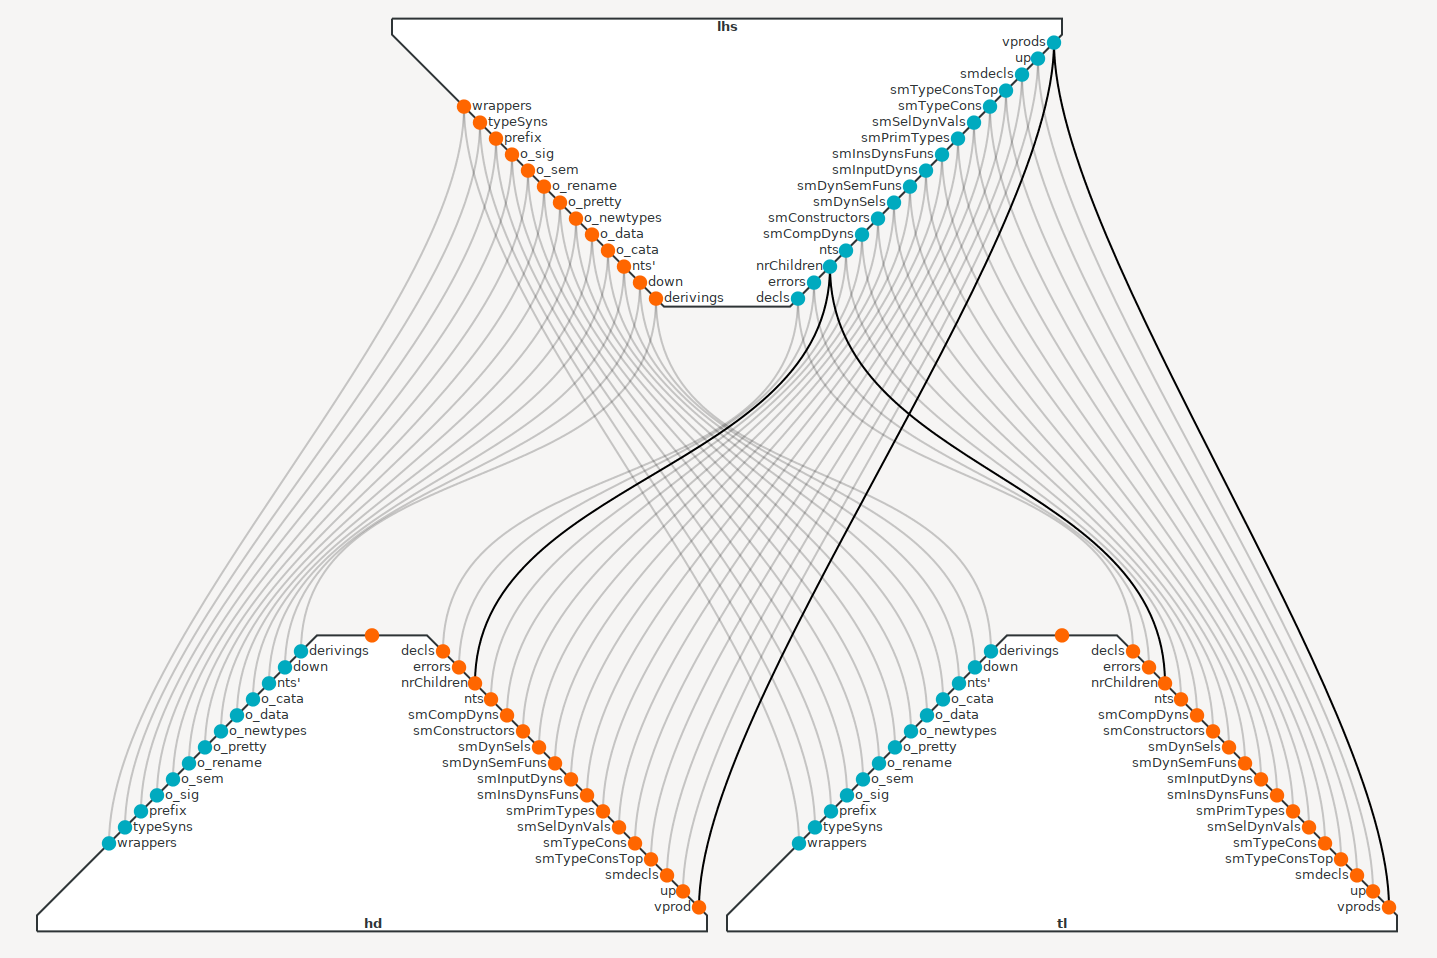
\includegraphics[width=\linewidth]{big-mirage}
  \caption{The big example from Figure~\ref{big-visage} visualized in Mirage.}
  \label{big-mirage}
\end{figure}

\subsection{Local attribute layout}

Another important element of some productions are local attributes. Local attributes are attributes that are not directly inherited or synthesized, but they can be used as intermediate variables to compute the value of other attributes. They can depend on attributes from the lhs or from the children, but also on other local attributes. In that way they form a free form graph structure between the lhs and the children. 

In Visage this graph structure is completely flattened and all the local attributes are placed next to each other to the right of the lhs node.  This can create a tangled mess of incoming and outgoing dependencies. An example of this is shown in Figure~\ref{locals-visage}; the local attributes are the yellow ellipses in the top right. It should also be noted that multiple local attributes can be declared together using a pattern, for example in a tuple. Visage creates virtual local attributes for these patterns to avoid showing many long lines to a group of local attributes, but it also introduces indirection and it takes up more space.

\begin{figure}[h]
  \centering
  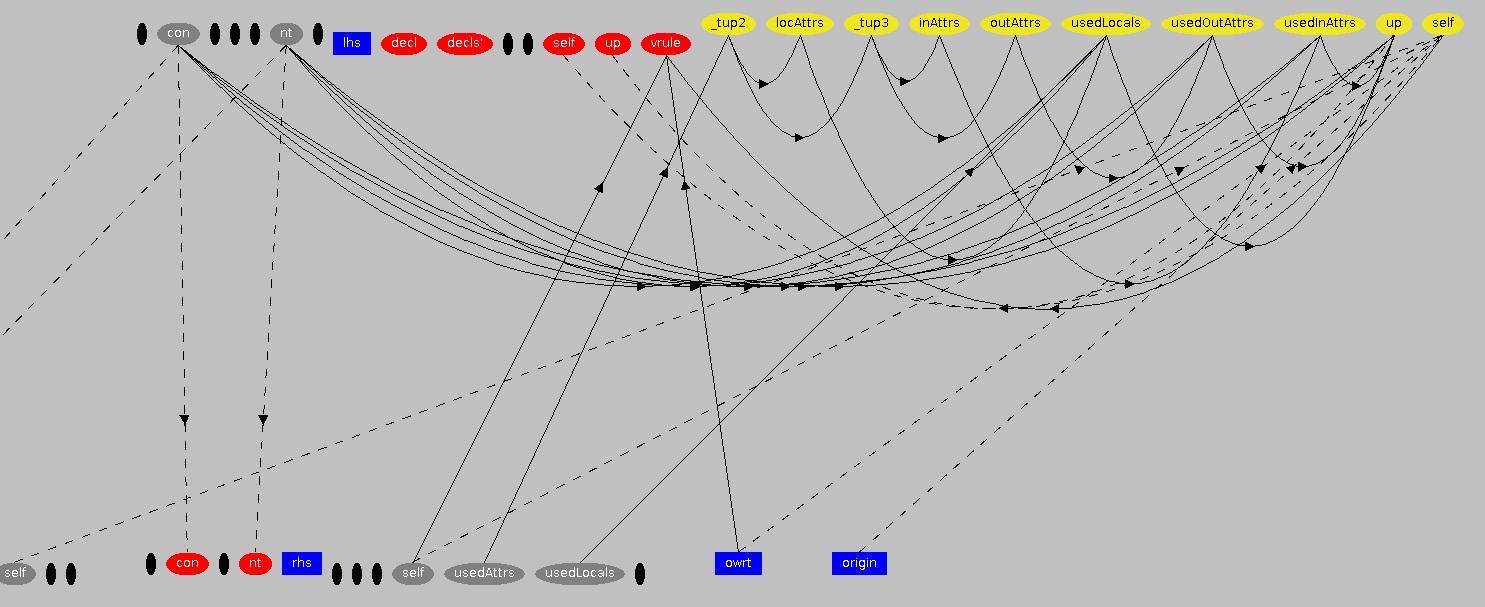
\includegraphics[width=\linewidth]{locals-visage}
  \caption{A production with many local attributes visualized with Visage. Some attributes that were not relevant to the local attributes are hidden.}
  \label{locals-visage}
\end{figure}

Mirage is a bit more flexible: it can place local attributes on both sides and in multiple rows. That should make it possible to retain a bit more of the graph structure and reduce the number of overlapping lines. Figure~\ref{locals-mirage} shows the same production as Figure~\ref{locals-visage}. Mirage places the local variables between the lhs node on top and the children on the bottom. The local variables are the octagonal shapes vertically in the center. In this example we see that some local attributes are placed on the left side and one local attribute is placed above the others on the right side. We currently compute the position of the attributes using a linear counting algorithm. If a majority of the connections of a local attribute is coming from the lhs or going to the children then it is placed on the left and otherwise it is placed on the right. A similar heuristic is used for placing the local attributes in multiple layers.

\begin{figure}[h]
  \centering
  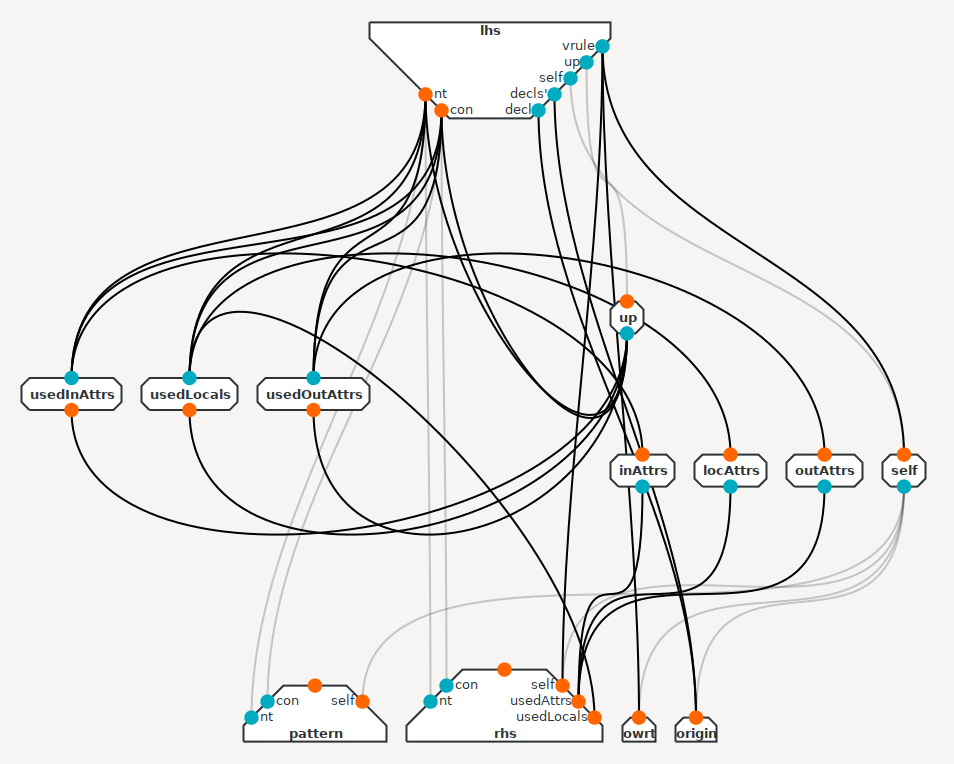
\includegraphics[scale=1.4]{locals-mirage}
  \caption{The same production with local attributes as Figure~\ref{locals-visage} with the same hidden attributes, but now visualized with Mirage.}
  \label{locals-mirage}
\end{figure}

\section{Implementation}

In addition to the final design discussed in Section~\ref{design}, we also want to give a look under the hood. One of the goals of this project was to improve maintainability of the code.
Mirage has been developed for the software technology research group at the University of Utrecht to visualize the attribute grammars of the Helium compiler. 
The group naturally spends most of its time on researching and developing new features of their compiler which leaves little time for maintenance. So, for this new tool to survive, its maintenance costs needs to be low.
In this section we describe measures that have been taken to achieve that.

\subsection{Haskell and UUAG}

Mirage is written in the Haskell and UUAG languages.
The UUAG compiler itself is also written in Haskell and UUAG.
That makes it possible to use the same or very similar data structures and exchange them with ease.
Furthermore, Haskell is designed to be easy to maintain and refactor due to its purity and immutability.
However, Haskell is not known for its good GUI programming capabilities.

\subsection{GUI programming with gi-gtk}

There are many competing GUI libraries, but not many are fully featured and not many have well maintained Haskell bindings.
Many contemporary GUI applications, in any language, even go as far as to render their user interface in a web browser.
An example of a Haskell library that has focused on this approach is Reflex\footnote{\url{https://reflex-frp.org/}}.
Using a web browser to render the GUI has the advantage of being very portable and web applications are often easier to write, but it also comes at the cost of consuming much more resources on the computers of the users.
We have opted to use GTK because it has the best maintained Haskell bindings, namely gi-gtk.
These bindings are automatically generated using metadata files provided by the upstream GTK library, which should make the Haskell bindings much easier to maintain.

There is one related library, Cairo, that does not have this metadata and hence has no automatically generated bindings.
It is still very important for us that Cairo is well supported because we use it for drawing the custom shapes of our visualization.
Luckily, there are handwritten bindings for this package in Haskell and this library does not have a very big API, so it should not be too difficult to maintain. In Section~\ref{custom-shapes} we explain further measures we have taken to make the dependency on Cairo smaller.

\subsection{Using an attribute grammar for rendering}

The core functionality of Mirage is to render a production of an attribute grammar to a nice image.
It involves walking over the abstract syntax tree and producing some parts of the image at every node.
To me, that sounds like the kind of problem where UUAGC can help, so I decided to try it out.

The current implementation has four attribute grammar files: \texttt{AbstractSyntax.ag}, \texttt{StaticInfo.ag}, \texttt{RenderShapes.ag} and \texttt{DependencyGraph.ag}.
In the file \texttt{AbstractSyntax.ag} we define the abstract syntax of attribute grammars and some other data types. This file can be included into other files to define different semantics that all work on the same types.

The first tree traversal is defined in \texttt{StaticInfo.ag}. It is intended to be computed once after loading an attribute grammar. It collects a list of all nonterminals and productions that the user can choose from and it also collects a list of attribute names that the user can disable and enable.

The main semantics are defined in \texttt{RenderShapes.ag}. In this traversal we determine the location, size and shape of all the visual elements. We also collect a map containing the locations of the disks of each attribute and we draw connections between them if one depends on the other.

In the rendering traversal we also use an advanced feature of UUAGC, namely higher-order attributes. This allows us to create a new child and traverse over it during the main traversal.
We use higher-order attributes in Mirage because all attributes are only stored in the nonterminals, and dependencies and local attributes first need to be computed from the rules.
We instantiate four higher-order attributes: a node for the lhs of a production, nodes for all the children, the local attributes and the dependencies.
After they have been computed they will be traversed in the same pass.
Without these higher-order attributes we would need to define two separate data structures and explicitly transform one into the other before rendering.

% TODO: Something about bounding box trees?

Finally, there is a traversal in  \texttt{DependencyGraph.ag}. That traversal is used to collect all dependencies in one big graph and that file also contains an operation that calculates the transitive closure of an attribute using the common semi-naive fixed-point algorithm. This file could and should probably be merged into the \texttt{StaticInfo.ag} file, but this has not been done yet.

\subsection{A custom shapes type}
\label{custom-shapes}

We discussed before how the Cairo library has to be maintained by hand and is therefore more susceptible to become unmaintained.
To prepare for this specifically, but also because it is good design in general, we have decided to reduce the dependency on Cairo as much as possible.
Concretely, in the rendering transformation we do not render directly to the screen.
We render to a shapes type that contains information about which shapes should be drawn at which positions.
Currently, the shapes type supports polygons for the nodes, disks for the attributes, text for the node and attribute names, and Bézier curves for the dependencies.
While rendering we produce a list of these shapes with concrete positions.
In the end we simply render each of those shapes to the screen with a very straightforward Cairo implementation.
So, if Cairo ends up being unusable then it should be simple to replace only that final rendering step with an implementation that uses another library.

An alternative would be to use the existing graphics EDSL called Diagrams~\footnote{\url{https://archives.haskell.org/projects.haskell.org/diagrams/}}.
Diagrams has a back-end for rendering with Cairo, but it is many times bigger than our custom backend and it is not very stable.
Perhaps if many applications start to use this same package then the maintenance burden could be shared, but we do not think that is the case right now.
This does mean that we have much fewer features and a less user-friendly API.

\subsection{Local attribute layout by counting}

In Section~\ref{design} we mentioned that we improve on Visage by displaying local attributes in multiple rows on both sides of the screen.
That requires an algorithm that determines on which side and in which row each local attribute should go.
There are many possible implementations, but for the initial version of Mirage we decided on a simple single-pass algorithm based on counting the dependencies of the local attributes.
We group the dependencies into three categories: connected with the lhs node, connected with the children, and connected with other local attributes.

Local attributes that have many dependencies that depend on the inherited attributes of the lhs and on which many inherited attributes of the children depend are moved to the left side of the screen.
Conversely, local attributes that depend on many synthesized attributes of the children and on which many synthesized attributes of the lhs depend are moved to the right side of the screen.
In the case of mixed connections we choose the side of the majority.
So, dependencies on local attributes are not used to determine the horizontal position. 

For even more simplicity we have chosen to limit the number of local attribute rows to two.
So, we simply have to decide if each local attribute should be closer to the children or closer to the lhs.
On the left side of the screen information flows downward from the lhs to the children.
So, we place local attributes on the bottom row that depend on many other attributes or on which many attributes of the children depend.
And, we place local attributes on the top row if many other attributes depend on it or if that attribute depends on many attributes of the lhs.
On the right side of the screen information flows upward from the children to the lhs, so we do the same but then with the top and bottom row switched.

\subsection{Modifying UUAGC}

I have also modified UUAGC itself such that it produces the information that we need to visualize the attribute grammars with Mirage.
However, modifications should be considered very carefully because UUAGC is already a big project and Mirage output is not one of its primary functions.

For Mirage, I only needed to add a very simple JSON output utility and an attribute grammar pass that generates JSON from the abstract syntax.
% TODO: I could go more into detail about the attribute grammar pass that generates JSON
Using a minimal JSON output utility on the side of UUAGC means that we do not need to add any dependencies, but we can still depend on the industrial strength JSON library called Aeson from the side of Mirage.
This is ideal because outputting JSON is easy and done on the UUAGC side.
Parsing JSON is harder, but we can use Aeson to automatically generate parsing functions for our data structures in Mirage.
And, even if we could add Aeson as a dependency in UUAGC, we would not even want to automatically generate the JSON output functions because we only want to export a subset of the data with some modifications.

\section{Conclusion}

In this report we described Mirage, a visualization tool for attribute grammars.
We give an overview of the main design decisions and compared it with an older visualization tool called Visage.
Mirage can visualize larger attribute grammars due to the trapezoidal node shapes, the improved layout of local attributes and the attribute filtering functionality.
Additionally, low-cost maintenance is one of the goals of Mirage.
So, we have discussed the most important implementation details and shown how they affect the maintainability of Mirage.
This description of the implementation can also serve as a high-level overview of Mirage for future maintainers and developers.
The source code can be found at \url{https://github.com/Helium4Haskell/mirage}.

But, the current version of Mirage is only the beginning of a visualization tool for attribute grammars. There are many possible features that were not implemented due to time constraints. In this section we will explain our ideas for features that could be implemented in the future. We have grouped the future work into a few general categories that are covered in no particular order.

\subsection{Future work}

First of all, the filtering of attributes can be improved. One major improvement would be to allow users to create attribute groups. This could be done by the user manually selecting attributes to group or automatically with some heuristics, for example using the number of dependencies or the name of the attribute. These groupings could be saved and loaded. A main developer of an attribute grammar could define these groupings so that other developers can focus on only the attributes from a certain group if they want to work on a certain feature.

\begin{figure}[h]
  \centering
  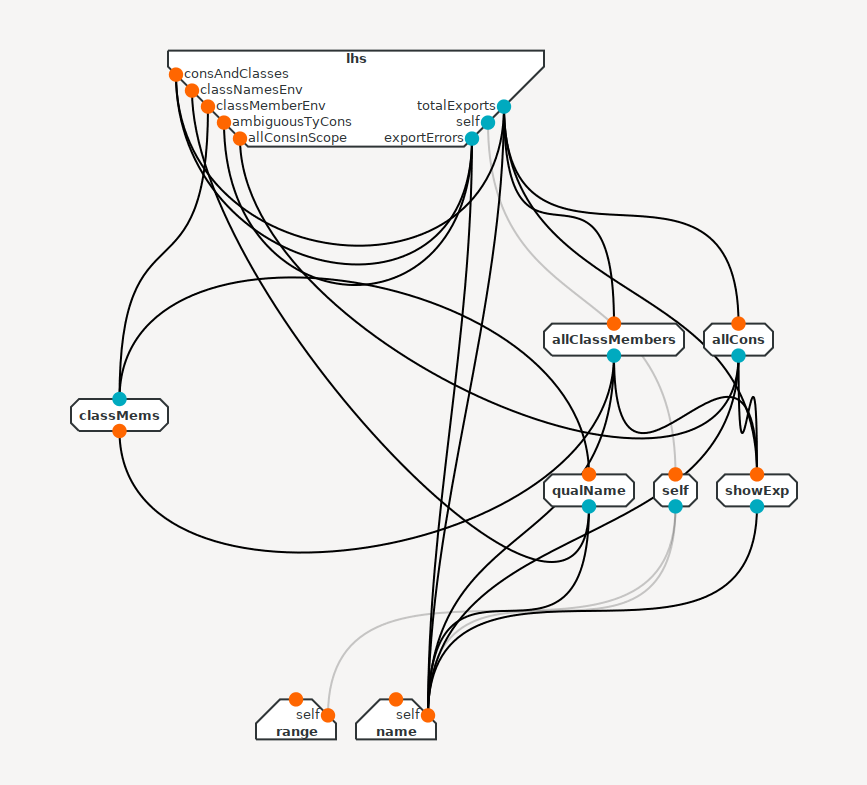
\includegraphics[scale=1.6]{inaccurate-locals-mirage}
  \caption{A production from the Helium compiler visualized with Mirage. This production shows inaccurate placing of the `classMems' attribute due to the linear layout algorithm.}
  \label{inaccurate-locals-mirage}
\end{figure}

Another category are improvements of the local attribute layout:
\begin{itemize}
  \item Currently, we use a simple linear counting algorithm, but that is not very accurate. See for example the `classMems' attribute in Figure~\ref{inaccurate-locals-mirage}. It is placed on the left side, but it has two connections to attributes on the right side, so it would be better to place it on the right side. A fixed-point algorithm that uses information about the positions of local attributes can certainly generate much better layouts in many cases.
  \item Users may also have their own preferences such as keeping most attributes on one side and only move attributes to the other side if those attributes really only are connected on that side. Another preference could be the weight of the connections on the layout, for example the connections to the lhs node could be set to a lower weight to make them have less influence on the final layout. 
  \item The layout could also be improved by allowing more than two rows or maybe even a completely free graph structure of the local attributes. A good graph layout could be found by a physical simulation of virtual springs connected to each of the local attributes.
\end{itemize}

\begin{figure}[h]
  \centering
  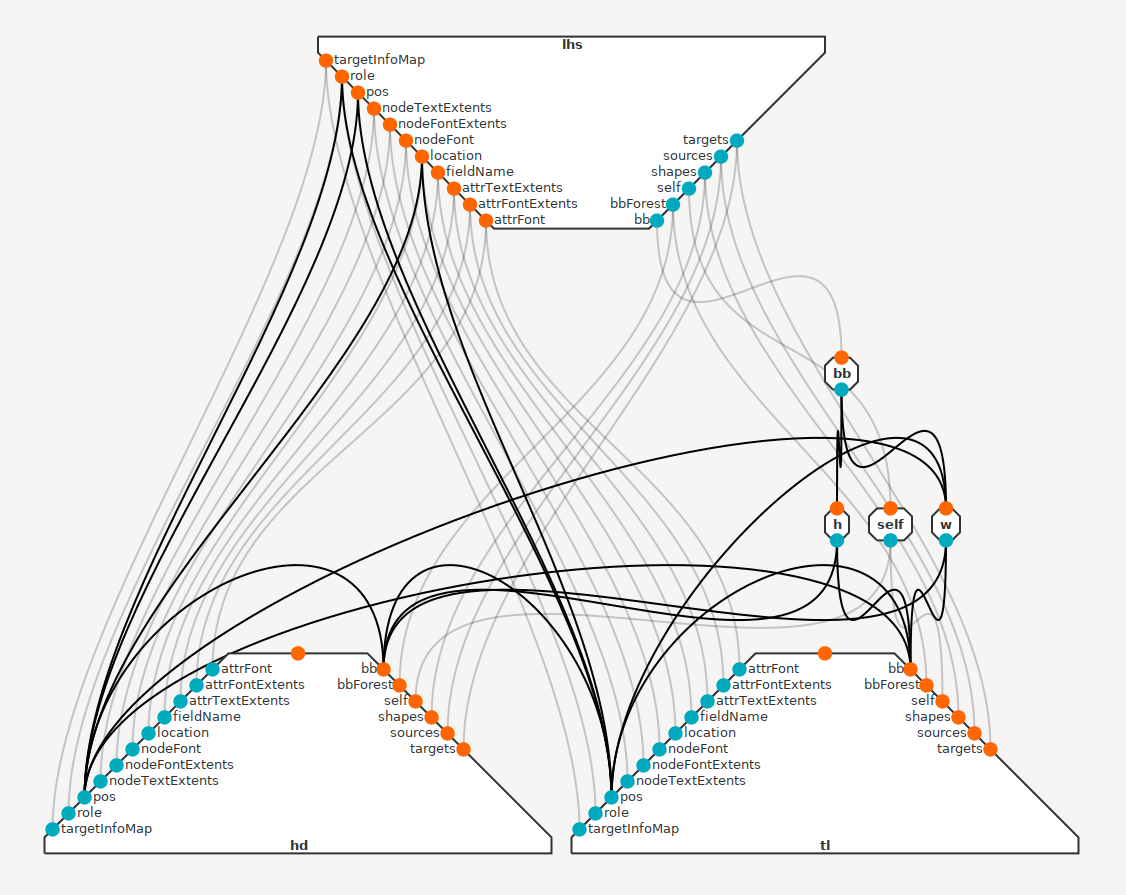
\includegraphics[width=\linewidth]{s-shape-mirage}
  \caption{A production of Mirage visualized with Mirage itself. This production shows that the connections can form ugly S-shapes if their endpoints are too close together.}
  \label{s-shape-mirage}
\end{figure}

Then, there are some visual improvements that could be made:
\begin{itemize}
  \item The simplest would be to change the disks of inherited attributes to directed triangles. These triangles could indicate the direction of the information flow. And these triangles would also improve the visual distinction between inherited and synthesized attributes.
  \item Another simple but useful change is to improve the Bézier curves that are used for the connections. Currently, the intermediate control points are always the same distance away from the endpoints. That causes a sideways S-shaped connection line if the endpoints get too close together. An example of this is shown in Figure~\ref{s-shape-mirage}, for example between the `bb' attribute of the `tl' child to the local attribute `w'. And this common distance also causes many lines to overlap with other lines, especially those that are connected to local attributes. We believe that slightly smarter rules for the placement of the control points could improve the visualization considerably in many cases.
  \item There are two situations in which we can hide more and in that way clean up the visualization. Firstly, if the user has filtered out all the attributes that are used in a production, then that production can be hidden in the list of productions in the sidebar. Secondly, if the user has hidden attributes such that there are some groups of local attributes in the current production that are not connected to the lhs or a child anymore, then those local attributes can be hidden. This could perhaps be combined with a fixed-point algorithm for the layout of the local attributes.
  \item We have considered making connections stand out by moving them in a wave like fashion. We expect that such movement makes it much easier to see the begin and endpoint of a connection when it crosses many other connections. This motion could perhaps be achieved without too much difficulty by slightly perturbing the intermediate control points of a connection.
\end{itemize}

The final category of relatively small changes concerns improvements in the interactivity of Mirage:
\begin{itemize}
  \item A very simple change would be to open the file that contains the implementation of an attribute definition in a text editor. Users could write a format string that contains a shell command that runs the editor of their choice which Mirage could interpolate with the file name and line number and then open the editor with that command.
  \item Another useful addition would be search functionality, especially for the filter lists but also the nonterminal and production list. In larger attribute grammars it can take long to find the attributes and nonterminals and productions that you are interested in.
  \item Another change would be to allow the user to hide attributes directly from the main visualization, then users would no longer need to open the filter window and look up the attribute name to do this common operation.
  \item Finally, a big and perhaps difficult change would be to allow the user to drag local attributes to a custom position. And it should be possible to persist this custom position.
\end{itemize}

A possible big change would be in the way that the user selects a nonterminal and production. Instead of the flat list of nonterminals and productions in the sidebar Mirage could show the parent-child relations between the nonterminals in a graph structure. That should make it easier to navigate the nonterminals and productions. But, that is not obvious and it is also not clear that the benefits are worth the cost to implement this.

There are also some changes to the implementation of Mirage, which do not introduce new features, that we would like to explore. A problem with the current implementation is that the GUI is implemented using an imperative interface which means that we lose many of the advantages of Haskell. There is a package named gi-gtk-declarative that adds a declarative API to the gi-gtk package. But, we have not used it for two reasons: it is not stable and it might not be actively maintained and developed in the near future, and secondly it does not support all features of GTK which means that it might need to be extended before it can be used by Mirage. Nevertheless, its declarative API could make the GUI code much more readable.

Finally, we would like to suggest possible future work on a different but related tool. Mirage can visualize static information about attribute grammars, but for debugging it can also be helpful to look at all the evaluated attributes of a specific tree. This requires extending the visualization. Currently, Mirage draws only a single level of each tree with a node and its children. That needs to be extended and the user needs to have some way to pan around to view all parts of the annotated abstract syntax tree and perhaps also zoom in and zoom out. But, the most uncertain part is how to get the evaluated values from a tree. This could be easy if an explicit tree is built up and stored as a Haskell value, but it also might be hard if intermediate values are discarded during the traversal.

\printbibliography
\end{document}
